\documentclass[TFG.tex]{subfiles}

\begin{document}


%\hyphenation{equi-va-len-cia}\hyphenation{pro-pie-dad}\hyphenation{res-pec-ti-va-men-te}\hyphenation{sub-es-pa-cio}
\chapter{Representaciones lineales}\label{capitulo4}

La existencia (o no existencia) de representaciones lineales fieles de los grupos de trenzas es una de las mayores cuestiones de esta área de investigación. Este problema fue por primera vez resuelto por Bigelow \cite{Bigelow} y Krammer \cite{Krammer} en el año 2000, mediante la conocida como \emph{representación LKB}. Además de esta representación existen otras, como la representación de Burau reducida, con la cual empezaremos este capítulo.

\section{Representación de Burau reducida}

%LA REDUCIDA MIRA LA IMAGEN DE $x_ix_{i+1}^{-1}$ 
%
%CURVA = FILA
%PUNTO = COLUMNA
%DERECHA = SIGNO POSITIVO
%EL PISO MÁS BAJO EN EL CAMBIO DE PISO TE DA EL EXPONENTE

\subsection{Definición a partir de espacios recubridores}

Consideremos el disco agujereado $n$ veces $\D_n$ con un punto base $d_0\in\D_n$. 
\begin{defi}
Para cada lazo $\alpha$ basado en $d_0$ denominamos \emph{índice total}  a la suma de los índices (número de vueltas) de $\alpha$ con respecto a cada agujero y lo denotamos $\phi\alpha$. Esto es, si un $\alpha$ está representado en $F_n$ por $\prod_{i=1}^k x_{j_i}^{m_{j_i}}$, entonces 
\[
\phi\alpha=\sum_{i=1}^{k}m_{j_i}.
\]
\end{defi}

Se observa que $\phi$ es un homomorfismo de grupos $\phi:\pi_1(\D_n)\to\Z$ al ser el índice total un invariante homotópico. Sea $\widetilde{\D}_n$ el espacio recubridor correspondiente a $\ker\phi$ (ver Definición \ref{corresponde}). Vamos a describir geométricamente este espacio recubridor (ver Figura \ref{recubrimiento}). 

%si es invariante homotópico también lo será por homeomorfismo

Para visualizarlo mejor, vamos a agrandar los agujeros de modo que se conviertan en bolas abiertas y llamamos a este nuevo espacio $X$. Dibujamos segmentos $A_1,\dots, A_n$ desde el centro de las bolas hasta el borde del disco. Cortamos $X$ a lo largo de estos segmentos, de modo que obtenemos dos copias disjuntas $A_i^+$ y $A_i^-$ de cada $A_i$. Llamamos a este espacio $X^*$. Sean $h_i:A_i^+\to A_i^-$ homeomorfismos y tomamos una cantidad numerable de copias $X^*_j$ de $X^*$. Para cada $j$ sea $g_j:X^*_j\to X^*$ un homeomorfismo. El espacio $\widetilde{X}$ se define como la unión disjunta de los $X^*_j$ identificando $A_i^+\subseteq X^*_j$ con $A_i^-\subseteq X^*_{j+1}$ mediante $g_{j+1}^{-1}h_ig_j$.

%a modo de gluing space, los A_i^signo están en X_j, por eso coges los g que te lo llevan a la copia adecuada

%Se idenfitica A_i^+ con la imagen mediante la aplicación esa
El hecho de que este sea el recubrimiento correspondiente a $\ker\phi$ se debe a que, fijada una preimagen $\tilde{d}_0\in\widetilde{X}$ de $d_0$, un lazo en $d_0$ se levanta a un lazo en $\tilde{d}_0$ si y solo si su índice total es nulo, pues para cada vuelta positiva sube un nivel en el recubrimiento y para cada vuelta negativa lo baja, así que para acabar de nuevo en $\tilde{d}_0$ deberá subir tantas veces como baja, es decir, que el número total de vueltas sea nulo.\\

\vspace{0.1cm}

\begin{figure}[h!]
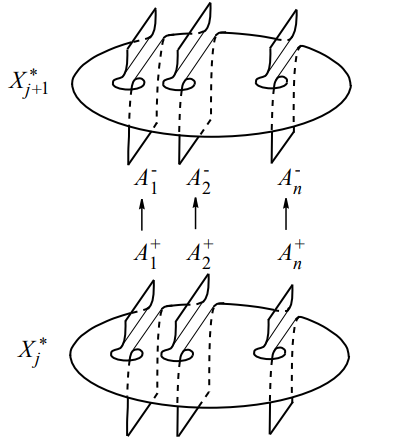
\includegraphics[scale=0.6]{Imagenes/recubrimiento}
\caption{Dos hojas del espacio recubridor $\widetilde{X}$.}\label{recubrimiento}
\end{figure}
Hay una acción natural de $\Z$ en $\widetilde{X}$ como transformación recubridora dada por $X^*_j\ni x\mapsto g_{j+n}^{-1}g_jx$ para cada $n\in\Z$. Esta acción se puede interpretar como cambiar el punto $x$ de nivel. Además, la acción es claramente libre y el espacio de órbitas $\widetilde{X}/\Z$ es $X$.%, por lo que el espacio recubridor es regular.


%PODRÍA DEFINIRLO ASÍ QUE ES MÁS SENCILLO EN LUGAR DE DEFINIRLO A PARTIR DE LAS TRANSFORMACIONES DE DECK QUE EMPIEZA COGIENDO AUTOMORFISMOS SOBRE LAS FIBRAS

%el espacio recubridor retrae con deformación sobre Z copias de n cuerdas con los extremos unidos a un mismo punto.


Vamos a ver cómo definir la representación de Burau reducida. Sea $\beta\in B_n$ inducida por un automorfismo $h$ de $\D_n$ que fija el borde punto a punto, lo cual vamos a denotar como $\beta=[h]$. Entonces, para cualquier lazo $\gamma$ en $\D_n$ se tiene que $\phi(h\gamma)=\phi\gamma$, de modo que $h$ induce una equivalencia de homotopía $\tilde{h}$ de $\widetilde{\D}_n$ que fija el borde \cite{Hatcher}. Pasando a la homología, esto nos da un automorfismo de $H_1(\widetilde{\D}_n)$. Si $h'$ es cualquier otro automorfismo con $[h']=\beta$, entonces $[h]^{-1}[h']=1$, así que como la aplicación inducida por el recubrimiento $\pi_1(\widetilde{\D}_n)\to\pi_1(\D_n)$ es inyectiva (\ref{inyect}) tenemos que $[\tilde{h}]^{-1}[\tilde{h}']=1$ como aplicación en $\pi_1(\widetilde{\D}_n)$. Pasando a homología, esto nos da $[\tilde{h}]^{-1}[\tilde{h}']=1$ como aplicación en $H_1(\widetilde{\D}_n)$. 

%EL SEGUNDO PASO A HOMOLOGÍA SE HACE ABELIANIZANDO CON HUREWICZ

%EL WINDING NUMBER ES INVARIANTE HOMOTÓPICO

%DE LO DE QUE PHI(H GAMMA)=PHI GAMMA SE OBTIENE QUE SI GAMMA ESTÁ EN EL KER DE PHI ENTONCES TAMBIÉN LO ESTÁ H(GAMMA)

%¿Se puede levantar siempre el automorfismo? Supongo que sí, porque $p:X->Dn, h:Dn->Dn$, entonces cojo para cada fibra $p^{-1}hp: X -> X$. Como en los segmentos coincide para cada fibra, se extiende a todo X. 


\begin{defi}
Sea el homomorfismo $\psi_r:B_n\to GL(H_1(\widetilde{\D}_n))$ dado por $\psi_r(\beta)=[\tilde{h}]$. Esta aplicación está bien definida por las observaciones anteriores y se conoce como \emph{representación de Burau reducida} de $B_n$.
\end{defi}

Se llama \emph{reducida} porque existe una representación $n$-dimensional de la cual la forma reducida es un sumando irreducible, es decir, que no se puede expresar como una combinación de dos representaciones lineales. Esta mencionada representación $n$-dimensional puede encontrarse en \cite{thesis}. Como veremos con la siguiente proposición, la representación que hemos dado es $(n-1)$-dimensional.

%SUMANDO IRREDUCIBLE: la reducida se expresa como suma directa de la reducida y de otra, lo cual se ve como que las matrices de la reducida son submatrices de las otras, de modo que la submatriz que dejan fuera no interactúa con las anteriores


\begin{prop}\label{dimension}
$H_1(\widetilde{\D}_n)$ es un módulo libre de rango $n-1$ sobre $\Z[t,t^{-1}]$.
\end{prop}
%módulo libre -> tiene base de longitud fija
%\begin{comment}
\begin{dem}
%El t es un generador de la homología del cociente ese que pone, luego tendrá winding number no nulo (si es generador imagino que 1 o -1), entonces eso lo que hace en el recubridor es subir y bajar pisos, además podemos coger solo un t porque todos los que tengan el mimso winding number están identificados. EN ESTA PRUEBA APARECE LO DE LOS GENERADORES $x_ix_{i+1}^{-1}$



Vamos a calcular la homología de $\widetilde{X}$, que es claramente del mismo tipo de homotopía que $\widetilde{\D}_n$. Además podemos considerar $\phi$ como una aplicación $\pi_1(X)\to\Z$ por ser $X$ homotópicamente equivalente a $\D_n$. Eligiendo entonces un generador $t\in \pi_1(X)/\ker\phi$ podemos ver $H_1(\widetilde{X})$ como un $\Z[t,t^{-1}]$-módulo, donde la suma se corresponde con la concatenación de lazos y el producto por $t$ con la conjugación por un lazo $x_i$. 

Sean $A=\bigcup_{j\in\Z}X_{2j}^*$ y $B=\bigcup_{j\in\Z}X_{2j+1}^*$ subespacios cuya unión es $\widetilde{X}$. La sucesión de Mayer-Vietoris nos da
\[
0\to H_1(\widetilde{X})\overset{\Delta}{\to} H_0(A\cap B)\overset{i_*}{\to} H_0(A)\oplus H_0(B),
\]
donde el 0 proviene de que $A$ y $B$ son homotópicamente equivalentes a un espacio discreto. Por tanto, $H_1(\widetilde{X})\cong \Ima\Delta=\ker i_*$. Ahora, $H_0(A\cap B)$ es isomorfo a $\bigoplus_{j\in\Z}\Z^n$, ya que para cada $j\in\Z$, la intersección $X_j^*\cap X_{j+1}^*$ es homotópicamente equivalente a un espacio de $n$ puntos. Entonces $\{a_{j,1},\dots, a_{j,n}\}_{j\in\Z}$ una $\Z$-base para $H_0(A\cap B)$. Es fácil ver que $\{a_{j,1}-a_{j,2},\dots,a_{j,n-1}-a_{j,n}\}_{j\in\Z}$ es una base para $\ker i_*$. Sea $\tilde{d}_0\in\widetilde{X}$ un levantamiento del punto base $d_0\in X$, digamos $\tilde{d}_0\in X_0^*$. Denotamos por $v_i$ el elemento de $H_1(\widetilde{X})$ representado por el levantamiento del lazo $x_ix_{i+1}^{-1}$ ($1\leq i\leq n-1$). Se tiene que $\Delta (v_i)=a_{0,i}-a_{0,i+1}$ \cite{thesis} y para todo $j\in\Z$ se tiene $\Delta(t^j v_i)=a_{j,i}-a_{j,i+1}$. Por tanto, los $t^jv_i$ forman una base de $H_1(\widetilde{X})$ como $\Z$-módulo, y como consecuencia $\{v_1,\dots, v_{n-1}\}$ es una base de $H_1(\widetilde{X})$ como $\Z[t,t^{-1}]$-módulo. \QED

\end{dem}
%\end{comment}

%Lo del t^j es que t es una que da solo una vuelta (se puede expresar como phi(p(t))=1, con lo cual en el recubridor sube o baja un nivel, así que hacer eso j veces te da j cambios de nivel y por eso te lo lleva a esa base

%el x_i que usemos para conjugar depende del v_i 

%Lo de que se corresponda al ker es como cuando en Hatcher hace corresponder un espacio recubridor de S1vS1 a cada grupo libre generado con combinaciones de los lazos ab. Como explica Hatcher, se hace cogiendo la imagen del homomorfismo inducido por el recubrimiento en el grupo fundamental del recubrimiento fijando un punto base preimagen del punto base de X. El subgrupo generado por esta imagen en pi(X,x0) es el que se corresponde con el recubrimiento. En este caso, fijada una preimagen de d0, los lazos en d0 son los que tienen total winding number 0 porque cada vez que hacen un giro bajan o suben de nivel, por lo que para volver a d0 tienen que subir lo mismo que bajan

%el homomorfismo inducido por el recubrimiento en los grupos fundamentales es siempre inyectivo (Hatcher)

%Over a commutative ring R, more care is needed: a matrix over R is invertible if and only if its determinant is a unit in R, that is, if its determinant is invertible in R. Therefore, GL(n, R) may be defined as the group of matrices whose determinants are units.

\begin{figure}[h!]
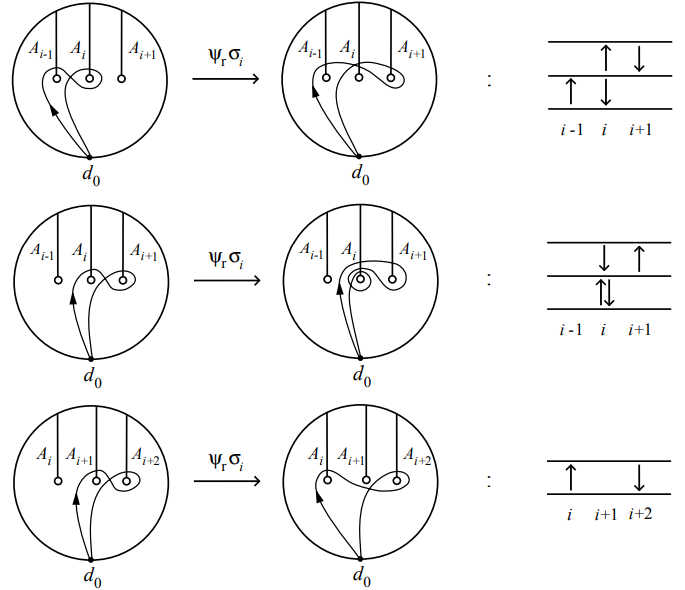
\includegraphics[scale=0.7]{Imagenes/Burau}
\caption{Acción de $\psi_r(\sigma_i)$ sobre $H_1(\widetilde{X})$.}\label{representacion}
\end{figure}

\subsection{Expresión matricial}
A partir de la demostración de la Proposición \ref{dimension} podemos obtener la expresión matricial de la representación de Burau reducida. Como explicaremos con ayuda de la Figura \ref{representacion}, la acción de $\sigma_i$ sobre $H_1(\widetilde{X})$ viene dada por

\[
\psi_r\sigma_i(v_j)=\begin{cases}
v_j+tv_{j+1} & j=i-1,\\
-tv_j & j=i,\\
v_{j-1}+v_j & j=i+1,\\
v_j & c.c.
\end{cases}
\]

Así, las matrices para la representación con respecto a la base $\{v_1,\dots, v_{n-1}\}$ son
\[
\psi_r(\sigma_1)=\begin{pmatrix}
-t & 0 & \\
1 & 1 & \\
& & I_{n-3}
\end{pmatrix}, \psi_r(\sigma_{n-1})=\begin{pmatrix}
I_{n-3} & &\\
& 1 & t \\
& 0 & -t 
\end{pmatrix},
\]
\[
\psi_r(\sigma_i )=\begin{pmatrix}
I_{i-2} & & &\\
& 1 & t & 0 & \\
& 0 & -t & 0 & \\
& 0 & 1 & 1 & \\
& & & & I_{n-i-2}  
\end{pmatrix}.
\]

Vamos a ver exactamente cómo obtener esta representación a partir de la Figura \ref{representacion}. Tenemos en la figura todos los casos en los que la acción de $\sigma_i$ afecta a un generador $v_j$ de $H_1(\widetilde{X})$ representado por un levantamiento de un lazo de la forma $x_jx_{j+1}^{-1}$. Buscamos expresar la imagen de cada $v_j$ como combinación con coeficientes en $\Z[t,t^{-1}]$ de la base de $H_1(\widetilde{X})$, para lo cual seguiremos la interpretación de $H_1(\widetilde{X})$ como $\Z[t,t^{-1}]$-módulo de la demostración de la Proposición \ref{dimension}. 
%Suponemos que partimos de la hoja $X^*_0$. Buscamos expresar el levantamiento la imagen de $x_jx_{j+1}^{-1}$ como el levantamiento de un conjugado de un producto de generadores del tipo $x_jx_{j+1}^{-1}$ y sus inversos. En la homología, conjugar no afecta porque es un grupo abeliano, pero nos indicará en qué nivel del recubridor comienza el levantamiento de cada $(x_jx_{j+1}^{-1})^{\pm 1}$. La fila en la que coloquemos los monomios será la $j$-ésima donde $x_jx_{j+1}^{-1}$ es el lazo al que se le aplicaba $\sigma_i$. La columna será la de índice $k$ tal que un levantamiento de $x_kx_{k+1}^{-1}$ (o de su inverso) es un factor del levantamiento de la imagen de $x_jx_{j+1}^{-1}$ mediante $\sigma_i$. El monomio que ocupará la posición $(j,k)$ será $(-1)^et^m$ donde $e$ es el exponente de $x_kx_{k+1}^{-1}$ y $m$ es el nivel más bajo del recubrimiento por el que pasa el levantamiento de $x_kx_{k+1}^{-1}$. El resto de entradas serán 0.
%

En el primer caso de la Figura \ref{representacion} partimos de $v_{i-1}$, y su imagen está representada por un levantamiento de $x_{i-1}x_ix_{i+1}^{-1}x_i^{-1}=(x_{i-1}x_i^{-1})(x_ix_ix_{i+1}^{-1}x_i^{-1})$, que representa a $v_i+tv_i$. 

En el segundo caso el generador es $v_i$. La imagen viene dada por el levantamiento de $x_ix_{i+1}x_i^{-1}x_i^{-1}=x_i(x_ix_{i+1}^{-1})^{-1}x_i^{-1}$, es decir, un representante de $-tv_i$. 

Por último, en el tercer caso la imagen de $v_{i+1}$ es un levantamiento de $x_ix_{i+2}^{-1}=(x_ix_{i+1}^{-1})(x_{i+1}x_{i+2}^{-1})$, que representa al elemento $v_i+v_{i+1}$.

En los casos en los que $\sigma_i$ no modifica el lazo $x_jx_{j+1}^{-1}$ es claro que la acción resultante es la identidad. 
%En el primer caso de la Figura \ref{representacion} partimos de $x_{i-1}x_i^{-1}$ y vemos que el resultado es un levantamiento de $x_{i-1}x_ix_{i+1}^{-1}x_i^{-1}$, o equivalentemente en la homología, de $x_{i-1}x_i^{-1}x_ix_{i+1}^{-1}$. La primera expresión nos permite ver que el lazo $x_ix_{i+1}^{-1}$ ocurre entre el nivel 1 y el 2, ya que $x_{i-1}$ sube a $X^*_1$ en el recubridor, para luego bajar a $X^*_0$ con $x_i^{-1}$. La segunda expresión hace ver que hay dos generadores interviniendo. Entonces, como el lazo al que le aplicábamos $\sigma_i$ era $x_{i-1}x_i^{-1}$, vamos a situarnos en la fila $i-1$ de la matriz. En la columna $i-1$ introducimos la información proporcionada por $x_{i-1}x_i^{-1}$ en el levantamiento. Como hemos explicado, este generador aparece levantado entre los niveles 0 y 1, por lo que elegimos el monomio $t^0=1$ para ocupar la posición $(i-1,i-1)$. En el caso de $x_ix_{i+1}^{-1}$, que determina la posición $(i-1,i)$, como este generador aparece entre los niveles 1 y 2, el monomio que elegimos es $t^1=t$. 
%
%En el segundo caso, la imagen viene dada por el levantamiento de $x_ix_{i+1}x_i^{-1}x_i^{-1}=x_i(x_ix_{i+1}^{-1})^{-1}x_i^{-1}$, es decir, un conjungado de $(x_ix_{i+1}^{-1})^{-1}$. Como ahora $\sigma_i$ actuaba sobre $x_ix_{i+1}^{-1}$, nos situamos en la fila $i$. Al empezar con $x_i$, vemos que el levantamiento de $(x_ix_{i+1}^{-1})^{-1}$ ocurre entre los niveles 1 y 2. Como además tiene exponente negativo, la posición $(i,i)$ estará ocupada por $-t$. 
%
%Por último, en el tercer caso la imagen es un levantamiento de $x_ix_{i+2}^{-1}=x_ix_{i+1}^{-1}x_{i+1}x_{i+2}^{-1}$. Análogamente a los casos anteriores, tenemos un 1 en la posición $(i+1,i+1)$ y otro 1 en la posición $(i+1,i+2)$. 
%
%En los casos en los que $\sigma_i$ no modifica el lazo $x_jx_{j+1}^{-1}$ también se puede seguir el mismo razonamiento para concluir que los bloques restantes forman matrices identidad. También en los casos extremos de $\sigma_1$ y $\sigma_{n-1}$ se hace de la misma manera.

Se puede comprobar directamente que las matrices anteriores satisfacen las relaciones de la presentación \ref{presentacion}. Un hecho interesante de esta representación es que se sabe que es fiel para $n\leq 3$ \cite{Birman} y que no es fiel para $n\geq 5$ \cite{Bil}\cite{LP}, pero el caso $n=4$ sigue siendo un problema abierto.

\section{Representación LKB}

Siguiendo \cite{Krammer}, denotamos $Ref_n$ al conjunto de pares de enteros $(i,j)$ tales que $1\leq i<j\leq n$. Claramente, el cardinal de $Ref_n$ es $\frac{n(n-1)}{2}$.

Sea $R$ un anillo conmutativo con unidad y $q,t\in R$ dos elementos invertibles. Sea \(V=\displaystyle\bigoplus_{s\in Ref_n}Rx_s\) el $R$-módulo libre de rango $\frac{n(n-1)}{2}$ con base $\{x_s\}_{s\in Ref_n}$. 

Krammer \cite{Krammer} define una acción $R$-lineal de $B_n$ sobre $V$ como sigue:


\begin{equation}\label{LKB}
\sigma_k(x_{i,j})=\begin{cases}
x_{i,j} & \textit{si }(k<i)\text{ o }(j<k),\\
x_{i-1,k}+(1-q)x_{i,j} & \text{si } (k=i-1),\\
tq(q-1)x_{i,i+1}+qx_{i+1,j} & \text{si }(k=i<j-1),\\
tq^2x_{i,j} & \text{si }k=i=j-1,\\
x_{i,j}+tq^{k-i}(q-1)^2x_{k,k+1} & \text{si }(i<k<j-1),\\
x_{i,j-1}+tq^{j-1}(q-1)x_{j-1,j} & \text{si }(i<k=j-1),\\
(1-q)x_{i,j}+qx_{i,j+1} & \text{si }(k=j),
\end{cases}
\end{equation}
donde $1\leq i<j\leq n$ y $k=1,\dots, n-1$. Que la acción de $\sigma_k$ es invertible y que se cumplen las relaciones de \ref{presentacion} se verifica mediante cálculo directo. Esta es la conocida como \emph{representación LKB} (Lawrence-Krammer-Bigelow) o \emph{representación de Krammer} de $B_n$.
%Lawrence la definió pero no pudo probar que era fiel

%Para dar la matriz habría primero que fijar un orden en Ref y ya está
\begin{teorema}
Sea $R=\R[t^{\pm 1}]$ y $0<q<1$. Entonces, la representación $B_n\to Aut(V)$ es fiel para todo $n\geq 1$.
\end{teorema}

La prueba de este teorema se encuentra en \cite{Krammer}.

%Rango=número de generadores libres

\subsection{Representación de Bigelow}
Existe un caso particular de la representación LKB encontrado independientemente por Bigelow \cite{Bil}, la cual se puede obtener usando $R=\Z[q^{\pm 1},t^{\pm 1}]$. La ventaja de esta representación es que tiene una interpretación geométrica mucho más clara, como veremos a continuación.

Consideremos $C=M_2(\D_n)/\Sigma_2$. Aquí, $\Sigma_2$ actúa sobre $M_2(\D_n)$ enviando $(x,y)$ a $(y,x)$. Se denotarán los puntos de $C$ como $\{x,y\}$ ya que al actuar $\Sigma_2$ no importa el orden. La proyección $M_2(\D_n)\to C$ que lleva $(x,y)$ a $\{x,y\}$ es claramente un recubrimiento de dos hojas. Sean $d_0$ y $d_0'$ dos puntos de $\partial\D_n$ lo bastante cercanos entre sí como para que no se crucen las hojas del recubridor. Tomamos $c_0=\{d_0,d_0'\}$ como punto base de $C$.

%Es sobreyectiva y continua porque la preimagen de un abierto es unión de dos abiertos simétricos y disjuntos porque no está la diagonal
%lo de cercanos es para asegurar que estén siempre en la misma hoja del recubridor PREGUNTAR ESTO

Sea $\alpha:[0,1]\to C$ un camino basado $c_0$. Este camino se puede levantar relativamente a $(d_0,d_0')$ como un par de caminos de la forma $(\alpha_1,\alpha_2)$, con $\alpha_1,\alpha_2:[0,1]\to\D_n$, el primero basado en $d_0$ y el segundo en $d_0'$. Denotemos pues $\alpha(t)=\{\alpha_1(t),\alpha_2(t)\}$. Nótese que si $\alpha$ es un lazo entonces $\{\alpha_1(0),\alpha_2(0)\}=\{\alpha_1(1),\alpha_2(1)\}=\{d_0,d_0'\}$. Por lo tanto, o bien $\alpha_1$ y $\alpha_2$ son ambos lazos o bien su concatenación forma un lazo. Ambos casos se observan en la Figura \ref{loop}. 



%en la figura se ve que se cortan, pero basta que no se corten para el mismo valor de t

Si $\alpha_1$ y $\alpha_2$ son caminos en $\D_n$ con $\alpha_1(t)\neq\alpha_2(t)$ para todo $t\in[0,1]$, entonces $(\alpha_1,\alpha_2)$ es un camino en $M_2(\D_n)$. La imagen de este camino mediante la proyección $M_2(\D_n)\to C$ se denota $\{\alpha_1,\alpha_2\}$.

\begin{figure}[h!]
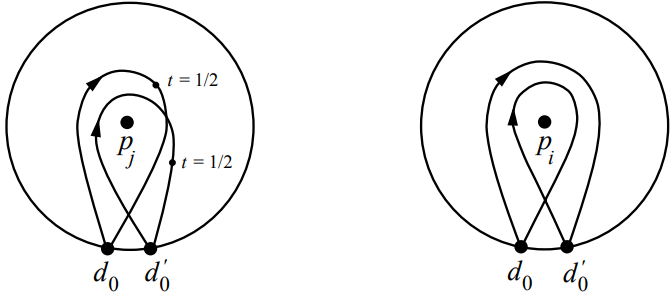
\includegraphics[scale=0.55]{Imagenes/loop}
\caption{A la izquierda, un lazo en $C$ que surge cuando los dos caminos originales son lazos (el parámetro $t$ muestra cómo está parametrizado el lazo). A la derecha, la concatenación de los dos lazos originales da lugar a un lazo en $C$.}\label{loop}
\end{figure}\ %el t tal como está puesto indica que aunque se crucen en el dibujo no es al mismo tiempo

Sea $\alpha:[0,1]\to C$ un representante de un elemento en $\pi_1(C)$. Se definen las aplicaciones $a,b:\pi_1(C)\to\Z$ como sigue: si $\alpha_1$ y $\alpha_2$ son ambos lazos, entonces $a(\alpha)$ es la suma de los índices totales de $\alpha_1$ y $\alpha_2$. Si no son ambos lazos, entonces $a(\alpha)$ es el índice total del lazo $\alpha_1\alpha_2$. La aplicación $b$ está definida en primer lugar componiendo $[0,1]\ni t\mapsto \dfrac{(\alpha_1(t)-\alpha_2(t))}{|\alpha_1(t)-\alpha_2(t)|}\in S^1$ con la proyección $S^1\to \R P^1$ para obtener un lazo en $\R P^1$. El correspondiente elemento de $H_1(\R P^1)\cong\Z$ es $b(\alpha)$. Por tanto, $a$ mide la cantidad de veces que los lazos $\alpha_1$ y $\alpha_2$ envuelven a los agujeros, mientras que $b$ mide las veces que un lazo envuelve al otro.

%SI RP ES HOMEOMORFO A S1, ¿PARA QUÉ PROYECTAR?: Si acaban en los puntos opuestos entonces en S1 saldría en el (-1,0) pero en RP1 ese punto y el (1,0) son el mismo. 

%LO DE B es que si coges el segmento que une dos puntos simultáneos de las curvas, se cuenta las veces que el segmento se da la vuelta (media vuelta basta por aquello del proyectivo, así es un lazo aunque solo dé media vuelta

Sea $\langle q,t\rangle$ el grupo libre abeliano  generado por $q$ y $t$. Se define la aplicación $\phi:\pi_1(C)\to\langle q,t\rangle$ mediante $\alpha\mapsto q^{a(\alpha)}t^{b(\alpha)}$. Por ejemplo, si en la Figura \ref{loop} denotamos al lazo de la izquierda $\gamma_1$ y al de la derecha $\gamma_2$, tenemos $\phi(\gamma_1)=q^2$ y $\phi(\gamma_2)=tq^2$. 

Sea $\widetilde{C}\to C$ el espacio recubridor correspondiente a $\ker\phi$ y elijamos un levantamiento $\tilde{c}_0\in\widetilde{C}$ de $c_0$. El grupo de homología $H_2(\widetilde{C})$ se puede considerar como un un $\Z[q^{\pm 1},t^{\pm 1}]$-módulo, donde el grupo $\langle t,q\rangle$ actúa sobre $\widetilde{C}$ como transformaciones recubridoras \cite{Bigelow}.

Sea $h$ un automorfismo de $\D_n$ que fije el borde punto a punto. Entonces $h$ induce un automorfismo denotado igual $h:C\to C$ dado por $h(\{x,y\})=\{h(x),h(y)\}$. Es claro que $h(c_0)=c_0$. Por tanto, este homeomorfismo se levanta de forma única a una equivalencia de homotopía $\tilde{h}:\widetilde{C}\to\widetilde{C}$ que fija $\tilde{c}_0$. Por tanto, $\tilde{h}$ induce un isomorfismo de $\Z[q^{\pm 1},t^{\pm 1}]$-módulos $\tilde{h}_*:H_2(\widetilde{C})\to H_2(\widetilde{C})$.


\begin{defi}
La representación $\kappa:B_n\to Aut(H_2(\widetilde{C}))$ inducida por $h\mapsto\tilde{h}_*$ se llama \emph{representación de Bigelow}.
\end{defi}

\begin{teorema}
La representación de Bigelow $\kappa:B_n\to Aut(H_2(\widetilde{C}))$ es fiel para todo $n\geq 1$.
\end{teorema}

Este resultado se prueba en \cite{Bil}. También por \cite{Bil} podemos tomar una base $\{v_{i,j}\in H_2(\widetilde{C})\}_{(i,j)\in Ref}$. Con esto, podemos establecer la equivalencia \cite{nundam} entre esta representación y la representación  \ref{LKB} como sigue:
\[
v_{i,j}=x_{i,j}+(1-q)\sum_{i<k<j}x_{k,j},\quad x_{i,j}=v_{i,j}+(q-1)\sum_{i<k<j}q^{k-i-1}v_{k,j}.
\]

%El punto base se fija porque está en el borde

\section{Solución al problema de la palabra}
Los resultados anteriores demuestran que los grupos de trenzas son grupos lineales. Una vez obtenida una representación lineal fiel, es inmediato resolver el problema de la palabra a partir de la expresión matricial: basta hacer el producto de las matrices que representan las letras de la palabra. Si el resultado de dicho producto es la matriz identidad, entonces la palabra representa el elemento trivial y recíprocamente.

Dado que el producto de matrices se puede calcular en tiempo polinomial sobre la dimensión de la matriz, este algoritmo puede ser bastante rápido, pero la aparición de polinomios en $t$ y $t^{-1}$ de tamaño y coeficientes arbitrarios en las entradas de las matrices puede ralentizarlo significativamente, especialmente para trenzas de longitud larga.


\begin{ej}
Vamos a ver un ejemplo de resolver el problema de la palabra con la representación de Burau reducida para $n=3$, caso para el que sabemos que la representación es fiel. Para cualquier otra representación la mecánica es la misma. Consideremos la palabra $\sigma_1\sigma_2\sigma_1^{-1}\sigma_2^{-1}$. En este caso, tenemos las matrices
\[
\psi_r(\sigma_1)=\begin{pmatrix}
-t&1 \\
0 & 1
\end{pmatrix},\quad \psi_r(\sigma_2)=\begin{pmatrix}
1&0 \\
t&-t
\end{pmatrix}.
\]
Para este caso necesitaremos también las inversas
\[
\psi_r(\sigma_1^{-1})=\psi_r(\sigma_1)^{-1}=\begin{pmatrix}
-t^{-1}&t^{-1} \\
0&1
\end{pmatrix},\quad \psi_r(\sigma_2^{-1})=\psi_r(\sigma_2)^{-1}=\begin{pmatrix}
1&0 \\
1&-t^{-1}
\end{pmatrix}.
\]
Ahora, basta realizar el producto matricial
\[
\begin{pmatrix}
-t&1 \\
0 & 1
\end{pmatrix}\begin{pmatrix}
1&0 \\
t&-t
\end{pmatrix}\begin{pmatrix}
-t^{-1}&t^{-1} \\
0&1
\end{pmatrix}\begin{pmatrix}
1&0 \\
1&-t^{-1}
\end{pmatrix}=
\begin{pmatrix}
-t& 1\\
-t& -t^{-1}+1
\end{pmatrix}.
\]
Como la matriz no es la identidad, la palabra no representaba el elemento neutro.
\end{ej}

\end{document}
%https://arxiv.org/pdf/math/0006202.pdf
%http://ms.mcmaster.ca/~boden/students/Smeltzer-MSc.pdf
%Creo que el de encima y el de debajo son el mismo
% HE ESCRITO LO DE ESTA EN KRAMMER http://www.numdam.org/article/SB_1999-2000__42__389_0.pdf Aquí comenta cuándo la de Burau es fiel y cuándo no y quiénes lo probaron
%La de Krammer sí es faithful siempre
%LKB http://wrap.warwick.ac.uk/90207/1/WRAP_Theses_Coles_2017.pdf 

%Este tiene buena pinta http://go.owu.edu/~chjackso/Papers/thesis.pdf